\chapter{Théorème de Liouville et flot hamiltonien}

\lectureoverview{Les équations de Hamilton ne se contentent pas de reformuler les équations du mouvement. Elles définissent un champ de vitesses dans l’espace des phases dont la divergence est nulle. Cette simple compensation constitue le théorème de Liouville : l’évolution hamiltonienne préserve le volume dans l’espace des phases. Nous allons y parvenir en suivant l’ordre qui en fait apparaître le sens---d’abord la conservation de l’énergie, puis les surfaces d’énergie constante, ensuite un fluide de conditions initiales possibles, et enfin le contraste entre un flot qui préserve le volume et un puits dissipatif. Ce même langage mène naturellement aux crochets de Poisson.}

\section{Pourquoi une autre formulation de la mécanique ?}

Le théorème que nous cherchons est l’équivalent classique continu des diagrammes d’états réversibles présentés au début du cours. Dans une loi discrète réversible, chaque état possède une flèche entrante et une flèche sortante. Le présent suffit à déterminer à la fois l’état suivant et l’état précédent. Une loi défectueuse envoie de nombreux états vers un même puits : l’avenir peut être déterminé, mais le passé n’est plus récupérable.

Le théorème de Liouville décrit ce qu’il advient de cette distinction lorsque l’ensemble des états est un espace des phases continu. L’expression qui remplace « une flèche entrante et une flèche sortante » est \emph{autant de flot entrant que de flot sortant}. Mais, avant de pouvoir lui donner un sens mathématique, nous devons reconstruire le flot à partir des équations de Hamilton.

Il y a là une énigme historique. Hamilton, Jacobi, Lagrange et Poisson ont élaboré des formulations complexes et remarquables de la mécanique classique sans connaître la théorie quantique, dans laquelle ces formulations allaient devenir indispensables. Newton avait un objectif concret : le mouvement des planètes. Lagrange et Hamilton avaient eux aussi des problèmes physiques à résoudre, mais ils ont exploré des analogies et des structures qui dépassaient largement le cadre d’une orbite particulière. L’action stationnaire en mécanique rappelait les principes du temps minimal en optique ; le mouvement des rayons et celui des particules pouvaient être exprimés dans des formes mathématiques parallèles. Ils simplifiaient, réorganisaient et unifiaient les équations parce que les structures elles-mêmes semblaient renfermer de la physique.

Nous savons aujourd’hui que cette intuition s’est révélée extraordinairement féconde. Sur le plan logique, de nombreux aspects de la mécanique classique peuvent se comprendre comme des limites de la mécanique quantique. Historiquement, l’ordre a été inverse : les structures classiques ont été découvertes en premier, et leur portée plus profonde n’est apparue que bien plus tard. Une plaisanterie provocatrice attribuée à Feynman faisait ressortir ce point en opposant les mathématiques poursuivies pour elles-mêmes à une physique contrainte par un partenaire extérieur : le monde physique. Cette plaisanterie n’est pas un argument, mais la distinction est utile : la beauté formelle compte ici parce que la nature fait sans cesse appel à ces structures formelles.

\begin{classroomqa}
  \audiencequestion{Newton avait-il la conception moderne de l’énergie cinétique, et
  d’où vient la notion d’énergie ?
  \lecturetimestamp{00:04:24--00:05:50}}
  \lecturerresponse{La mécanique de Newton s’organisait autour de la force et du mouvement,
  et non autour d’un principe général de conservation de l’énergie déjà abouti. La priorité historique exacte
  n’est pas tranchée dans la discussion. La \emph{vis viva} de Leibniz,
  \(\sum_i m_i v_i^2\), en fut un précurseur important et vaut deux fois l’énergie cinétique
  moderne. Les travaux ultérieurs sur la chaleur ont placé au premier plan sa conversion en travail mécanique.
  Les premières théories du calorique traitaient la chaleur comme une substance conservée ; l’idée moderne de formes
  d’énergie interchangeables ne s’est donc imposée que progressivement.}
\end{classroomqa}

\section{Équations de Hamilton et conservation de l’énergie}

Considérons un système doté de \(n\) paires canoniques,
\begin{equation}
  (q_i,p_i),\qquad i=1,\ldots,n.
  \label{eq:l7-canonical-pairs}
\end{equation}
À chaque coordonnée correspond une quantité de mouvement, et à chaque quantité de mouvement une coordonnée. La loi du mouvement est regroupée dans une seule fonction,
\begin{equation}
  H=H(q_1,\ldots,q_n,p_1,\ldots,p_n,t),
  \label{eq:l7-hamiltonian}
\end{equation}
et les équations de Hamilton s’écrivent
\begin{equation}
  \boxed{
  \dot q_i=\frac{\partial H}{\partial p_i},
  \qquad
  \dot p_i=-\frac{\partial H}{\partial q_i}.}
  \label{eq:l7-hamilton-equations}
\end{equation}
Le signe fait partie de la structure canonique. L’équation en \(q\) comporte le signe plus ; celle en \(p\) comporte le signe moins.

\begin{figure}[htbp]
  \centering
  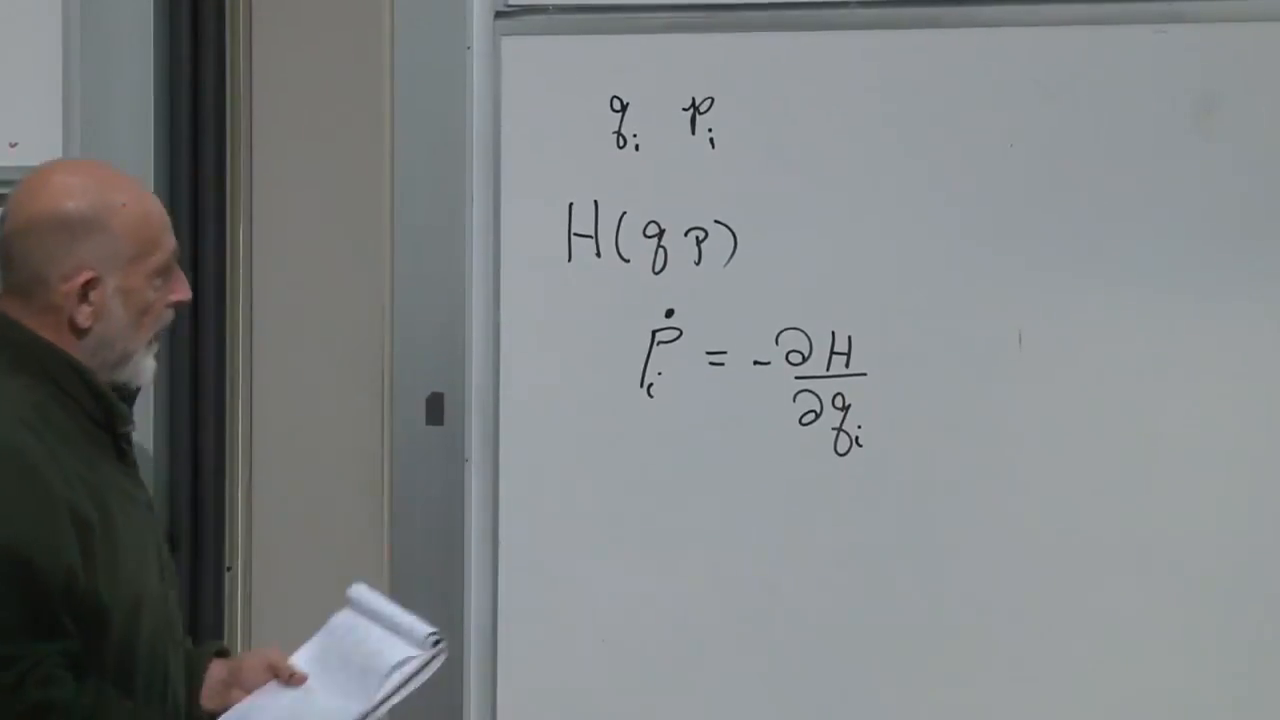
\includegraphics[width=0.82\textwidth]{lecture_07_figure_02.png}
  \caption{Les variables canoniques, la fonction \(H(q,p)\) et l’équation de Hamilton portant sur la quantité de mouvement, au début du récapitulatif.}
  \lectureframe{00:07:29}
\end{figure}

Bien que les équations soient organisées en paires indicées, la dynamique ne se sépare pas nécessairement paire par paire. Le Hamiltonien peut coupler tous les \(q_i\) et les \(p_i\) ; ainsi,
\(\dot p_1\), par exemple, peut dépendre de l’état du système tout entier.

\begin{classroomqa}
  \audiencequestion{La présentation est-elle maintenant axiomatique ? Quelle relation entre
  \(p\) et \(q\) a-t-on supposée ?
  \lecturetimestamp{00:17:08--00:18:18}}
  \lecturerresponse{Les équations de Hamilton définissent la théorie formelle dès lors que
  \(H(q,p)\) et les paires canoniques sont spécifiés. Il n’existe pas d’hypothèse supplémentaire
  universelle \(p=m\dot q\). Cette relation vaut pour une particule cartésienne ordinaire à énergie cinétique quadratique,
  mais d’autres coordonnées et d’autres Hamiltoniens donnent d’autres relations entre quantité de mouvement--et vitesse. Les équations elles-mêmes fournissent la relation par
  \(\dot q_i=\partial H/\partial p_i\). La question de savoir si un Hamiltonien proposé est réalisé dans la nature
  est une question physique distincte.}
\end{classroomqa}

Nous pouvons maintenant retrouver la conservation de l’énergie en un seul raisonnement. Le long d’une trajectoire, la dérivée totale de \(H\) vaut
\begin{equation}
  \frac{dH}{dt}
  =
  \sum_i\left(
    \frac{\partial H}{\partial q_i}\dot q_i
    +\frac{\partial H}{\partial p_i}\dot p_i
  \right)
  +\frac{\partial H}{\partial t}.
  \label{eq:l7-total-h-derivative}
\end{equation}
Le dernier terme représente la dépendance explicite en temps à \(q\) et \(p\) fixés, par exemple lorsqu’un paramètre imposé de l’extérieur varie. En substituant l’équation~\eqref{eq:l7-hamilton-equations},
\begin{align}
  \frac{dH}{dt}
  &=
  \sum_i\left[
    \frac{\partial H}{\partial q_i}
    \frac{\partial H}{\partial p_i}
    -\frac{\partial H}{\partial p_i}
    \frac{\partial H}{\partial q_i}
  \right]
  +\frac{\partial H}{\partial t}\\
  &=\frac{\partial H}{\partial t}.
  \label{eq:l7-h-energy-rate}
\end{align}
Chaque terme de la somme s’annule avec son correspondant. Par conséquent,
\begin{equation}
  \frac{\partial H}{\partial t}=0
  \quad\Longrightarrow\quad
  \frac{dH}{dt}=0.
  \label{eq:l7-energy-conservation}
\end{equation}
Pour un système fermé invariant par translation dans le temps, le Hamiltonien est conservé et correspond à l’énergie.

\begin{classroomqa}
  \audiencequestion{Que se passe-t-il si le Hamiltonien dépend explicitement du temps ? \lecturetimestamp{00:10:32--00:12:33}}
  \lecturerresponse{L’équation~\eqref{eq:l7-h-energy-rate} reste alors valable, mais l’énergie du sous-système
  n’est pas nécessairement constante. Une dépendance explicite en temps représente généralement un dispositif extérieur omis, qui échange de l’énergie avec le système. Si l’on inclut ce dispositif comme partie dynamique d’un système fermé plus vaste, le Hamiltonien global peut à nouveau être indépendant du temps et son énergie totale conservée.}
\end{classroomqa}

\section{L’énergie comme géométrie dans l’espace des phases}

Supposons maintenant que \(H\) ne dépende pas explicitement du temps. La condition initiale fixe une valeur \(E\), et le point représentatif dans l’espace des phases reste sur
\begin{equation}
  H(q,p)=E.
  \label{eq:l7-energy-surface}
\end{equation}
L’espace des phases a \(2n\) dimensions. Aux points réguliers, une équation entre ses coordonnées définit une hypersurface de dimension \((2n-1)\). Des valeurs différentes de \(E\) donnent des hypersurfaces différentes. Elles ne sont pas nécessairement fermées ou compactes ; la conservation de l’énergie signifie seulement qu’une trajectoire qui commence sur l’une d’elles ne la quitte jamais.

Pour l’oscillateur harmonique adapté du cours précédent,
\begin{equation}
  H=\frac{\omega}{2}(p^2+q^2).
  \label{eq:l7-oscillator-hamiltonian}
\end{equation}
Ainsi, chaque ensemble d’énergie constante est un cercle,
\begin{equation}
  p^2+q^2=\frac{2E}{\omega}.
  \label{eq:l7-oscillator-circle}
\end{equation}

\begin{figure}[htbp]
  \centering
  \includegraphics[width=0.84\textwidth]{lecture_07_figure_04.png}
  \caption{Schéma de l’espace des phases de dimension \(2n\) et Hamiltonien de l’oscillateur harmonique utilisés pour introduire les surfaces d’énergie constante.}
  \lectureframe{00:15:20}
\end{figure}

Les équations du mouvement,
\begin{equation}
  \dot q=\omega p,\qquad \dot p=-\omega q,
  \label{eq:l7-oscillator-flow}
\end{equation}
font tourner le point dans le sens horaire autour de son cercle. L’équation de l’énergie indique quelle courbe contient le mouvement ; les équations de Hamilton en donnent la direction et la vitesse le long de cette courbe.

\begin{figure}[htbp]
  \centering
  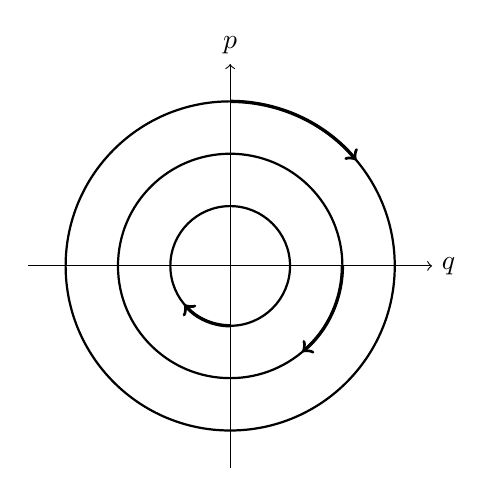
\begin{tikzpicture}[scale=0.95]
    \draw[->] (-2.7,0) -- (2.7,0) node[right] {\(q\)};
    \draw[->] (0,-2.7) -- (0,2.7) node[above] {\(p\)};
    \draw[thick] (0,0) circle (0.8);
    \draw[thick] (0,0) circle (1.5);
    \draw[thick] (0,0) circle (2.2);
    \draw[->,very thick] (0,2.2) arc[start angle=90,end angle=40,radius=2.2];
    \draw[->,very thick] (1.5,0) arc[start angle=0,end angle=-50,radius=1.5];
    \draw[->,very thick] (0,-0.8) arc[start angle=-90,end angle=-140,radius=0.8];
  \end{tikzpicture}
  \caption{L’énergie constante détermine les cercles ; les équations de l’oscillateur déterminent le champ tangent orienté dans le sens horaire.}
\end{figure}

\begin{classroomqa}
  \audiencequestion{Les deux équations de Hamilton et \(H=E\) sont-elles plusieurs formes d’une même équation ?
  \lecturetimestamp{00:15:53--00:17:06}}
  \lecturerresponse{Non. Les équations de Hamilton sont les deux lois du mouvement du premier ordre pour une paire canonique. Elles impliquent que \(dH/dt=0\), d’où découle \(H=E\). La valeur de \(E\) est déterminée par la condition initiale.
  L’équation \(H=E\) identifie une surface ; à elle seule, elle ne spécifie pas la vitesse le long de cette surface.}
\end{classroomqa}

\section{D’un état unique à un flot d’états}

Au lieu de suivre une seule condition initiale, parsemons l’espace des phases de toutes les conditions initiales possibles, puis lançons l’horloge. Chaque point représente un état possible complet, et chaque état évolue selon les équations de Hamilton. On peut imaginer cet ensemble comme une poussière ou un fluide fictif. Rien de matériel n’est versé dans l’espace des phases ; cette image du fluide permet de visualiser simultanément toutes les trajectoires.

Le champ de vitesses dans l’espace des phases est
\begin{equation}
  \mathbf V(q,p,t)
  =
  (\dot q_1,\ldots,\dot q_n,\dot p_1,\ldots,\dot p_n).
  \label{eq:l7-phase-velocity}
\end{equation}
Pour une seule paire canonique, nous écrivons
\begin{equation}
  V_q=\dot q=\frac{\partial H}{\partial p},
  \qquad
  V_p=\dot p=-\frac{\partial H}{\partial q}.
  \label{eq:l7-phase-components}
\end{equation}
En chaque point, le Hamiltonien attribue un vecteur qui indique au point représentatif où aller ensuite. Si \(H\) est indépendant du temps, le champ de vecteurs est stationnaire : lorsqu’on revient au même point de l’espace des phases, on retrouve la même vitesse. Si \(H\) dépend du temps, le champ lui-même varie au cours du temps, mais il reste défini à chaque instant.

\begin{figure}[htbp]
  \centering
  \includegraphics[width=0.84\textwidth]{lecture_07_figure_05.png}
  \caption{Le champ de vitesses de l’oscillateur harmonique. Les vecteurs sont tangents aux cercles et leur longueur diminue à mesure que l’on se rapproche de l’origine.}
  \lectureframe{00:24:50}
\end{figure}

Dans le cas de l’oscillateur harmonique, chaque rayon tourne à la vitesse angulaire \(\omega\). Les points proches de l’origine ont une vitesse linéaire plus faible, car ils parcourent un cercle plus petit pendant la même période. Toute la poussière tourne donc comme un carrousel rigide.

\begin{classroomqa}
  \audiencequestion{Une rotation rigide signifie-t-elle que toutes les trajectoires de l’oscillateur ont la même période ? \lecturetimestamp{00:21:10--00:21:42}}
  \lecturerresponse{Oui. L’indépendance par rapport à l’amplitude est la propriété caractéristique de l’oscillateur harmonique. Chaque cercle est parcouru avec la même pulsation \(\omega\), même si la norme de la vitesse dans l’espace des phases est plus faible sur un cercle plus petit.}
\end{classroomqa}

\begin{classroomqa}
  \audiencequestion{La vitesse dans l’espace des phases est-elle la même en tout point ?
  \lecturetimestamp{00:24:29--00:25:37}}
  \lecturerresponse{Non. Sa direction comme sa norme varient généralement avec la position. Pour l’oscillateur, le vecteur est tangent au cercle local et sa norme vaut \(\omega\sqrt{p^2+q^2}\). Un champ de vecteurs signifie qu’un vecteur est attribué à chaque point, et non qu’un même vecteur identique est reproduit partout.}
\end{classroomqa}

\begin{classroomqa}
  \audiencequestion{Que sont exactement les particules et la densité de ce fluide fictif ? \lecturetimestamp{00:56:03--00:58:40}}
  \lecturerresponse{Chaque point représente un état complet du système mécanique tout entier. Ce n’est pas une particule physique. Cinq particules se déplaçant dans une dimension spatiale requièrent cinq positions et cinq quantités de mouvement, donc un espace des phases à dix dimensions ; en trois dimensions, il en faut trente. La poussière représente un ensemble d’états possibles alternatifs. Si l’image du fluide vous gêne, considérez simplement une région de conditions initiales, faites évoluer chacun de ses points, puis comparez son volume dans l’espace des phases avant et après l’évolution.}
\end{classroomqa}

\section{Compression et divergence}

Pour savoir si ce fluide fictif perd du volume, commençons en une dimension. Des points sur une droite se déplacent avec la vitesse \(v(x)\). Deux points voisins séparés par \(\delta x\) présentent une différence de vitesse égale à
\begin{equation}
  \delta v \simeq \frac{dv}{dx}\,\delta x.
  \label{eq:l7-one-dimensional-strain}
\end{equation}
Si \(dv/dx>0\), le point situé devant se déplace plus vite et l’intervalle s’étire. Si \(dv/dx<0\), il se comprime. Un flot stationnaire incompressible à une dimension vérifie donc
\begin{equation}
  \frac{dv}{dx}=0.
  \label{eq:l7-one-dimensional-incompressible}
\end{equation}

\begin{figure}[htbp]
  \centering
  \includegraphics[width=0.84\textwidth]{lecture_07_figure_06.png}
  \caption{Construction en une dimension menant à \(dv/dx\) comme taux local d’étirement ou de compression.}
  \lectureframe{00:30:20}
\end{figure}

Deux points de vue équivalents sont possibles. Nous pouvons suivre un intervalle matériel et demander si sa longueur change. Ou bien nous pouvons maintenir un petit intervalle fixe et demander si la quantité qui y entre par unité de temps est égale à celle qui en sort. Le premier point de vue suit le fluide ; le second le voit passer.

En dimension supérieure, une région peut s’étirer le long d’un axe et se comprimer le long d’un autre sans que son volume total change. Pour un champ de vitesses \(\mathbf V=(V_x,V_y,V_z)\), le taux local pertinent est la divergence,
\begin{equation}
  \nabla\cdot\mathbf V
  =
  \frac{\partial V_x}{\partial x}
  +\frac{\partial V_y}{\partial y}
  +\frac{\partial V_z}{\partial z}.
  \label{eq:l7-spatial-divergence}
\end{equation}
Une divergence positive correspond à une expansion locale, une divergence négative à une contraction locale, et l’incompressibilité à
\begin{equation}
  \nabla\cdot\mathbf V=0.
  \label{eq:l7-zero-divergence}
\end{equation}
L’égalité des flux entrant et sortant à travers une petite boîte fixe exprime localement la même chose que la conservation du volume d’une petite boîte en mouvement.

\begin{figure}[htbp]
  \centering
  \includegraphics[width=0.86\textwidth]{lecture_07_figure_07.png}
  \caption{Boîte bidimensionnelle, composantes du flot et somme des dérivées par rapport aux coordonnées correspondantes qui définit la divergence.}
  \lectureframe{00:35:30}
\end{figure}

\begin{classroomqa}
  \audiencequestion{Parlons-nous d’un fluide dans l’espace ordinaire ou d’un flot dans l’espace des phases ? \lecturetimestamp{00:34:27--00:34:40}}
  \lecturerresponse{L’argument sur la divergence est d’abord un argument général sur les fluides. Nous l’appliquerons à l’espace des phases, de dimension paire, dont les directions de coordonnées sont les \(q_i\) et les \(p_i\), et dont les composantes de vitesse sont les \(\dot q_i\) et les \(\dot p_i\).}
\end{classroomqa}

Revenons maintenant aux applications discrètes entre états. Dans un cycle réversible, chaque nœud possède une flèche entrante et une flèche sortante, et un ensemble choisi d’états conserve le même nombre d’éléments au cours de son évolution. Dans un puits, de nombreuses flèches entrent et trop peu en sortent ; plusieurs possibilités deviennent indiscernables.

\begin{figure}[htbp]
  \centering
  \includegraphics[width=0.80\textwidth]{lecture_07_figure_08.png}
  \caption{Le puits discret qui relie la divergence au critère des lois réversibles présenté dans la première leçon.}
  \lectureframe{00:40:15}
\end{figure}

La question continue est maintenant précise : le flot hamiltonien a-t-il une divergence nulle, de sorte qu’une petite région d’états discernables ne soit jamais réduite à un volume plus petit dans l’espace des phases ?

\section{Théorème de Liouville}

\begin{theorem}[Liouville's theorem]Pour un système hamiltonien régulier, le champ canonique de vitesses dans l’espace des phases est de divergence nulle :
\begin{equation}
  \sum_i\left(
    \frac{\partial\dot q_i}{\partial q_i}
    +\frac{\partial\dot p_i}{\partial p_i}
  \right)=0.
  \label{eq:l7-liouville-divergence}
\end{equation}
De façon équivalente, l’évolution hamiltonienne préserve l’élément de volume canonique dans l’espace des phases
\(dq_1\cdots dq_n\,dp_1\cdots dp_n\).
\end{theorem}

\begin{classroomqa}
  \audiencequestion{Les composantes notées \(V\) sont-elles simplement les dérivées temporelles de \(p\) et de \(q\) ? \lecturetimestamp{00:42:20--00:43:22}}
  \lecturerresponse{Oui. Pour une paire,
  \(V_q=\dot q\) et \(V_p=\dot p\). En réunissant toutes ces dérivées, on obtient le vecteur vitesse du flot dans l’espace des phases tout entier.}
\end{classroomqa}

Pour une paire canonique, les équations de Hamilton donnent
\begin{equation}
  V_p=-\frac{\partial H}{\partial q},
  \qquad
  V_q=\frac{\partial H}{\partial p}.
  \label{eq:l7-liouville-components}
\end{equation}
La divergence vaut donc
\begin{align}
  \frac{\partial V_p}{\partial p}
  +\frac{\partial V_q}{\partial q}
  &=
  -\frac{\partial}{\partial p}
    \left(\frac{\partial H}{\partial q}\right)
  +\frac{\partial}{\partial q}
    \left(\frac{\partial H}{\partial p}\right)\\
  &=
  -\frac{\partial^2H}{\partial p\,\partial q}
  +\frac{\partial^2H}{\partial q\,\partial p}
  =0.
  \label{eq:l7-liouville-proof}
\end{align}

\begin{figure}[htbp]
  \centering
  \includegraphics[width=0.86\textwidth]{lecture_07_figure_09.png}
  \caption{Rectangle de différences finies utilisé pour expliquer pourquoi les dérivées partielles mixtes de fonctions régulières commutent.}
  \lectureframe{00:47:30}
\end{figure}

L’égalité des dérivées partielles mixtes se voit en considérant quatre points voisins \(A,B,C,D\) aux sommets d’un petit rectangle dans le plan \(q\)-\(p\). Calculer une différence selon \(q\), puis une différence selon \(p\), donne, à un facteur égal au produit des deux petits côtés près,
\begin{equation}
  F(B)+F(D)-F(A)-F(C).
  \label{eq:l7-finite-difference-combination}
\end{equation}
Prendre les différences dans l’ordre inverse donne la même combinaison. À la limite d’un rectangle infiniment petit, on obtient
\(\partial_p\partial_qF=\partial_q\partial_pF\), à condition que les dérivées requises soient continues.

\begin{figure}[htbp]
  \centering
  \includegraphics[width=0.88\textwidth]{lecture_07_figure_10.png}
  \caption{La divergence canonique, une fois les équations de Hamilton ramenées à deux dérivées mixtes de signes opposés.}
  \lectureframe{00:50:20}
\end{figure}

Pour de nombreux degrés de liberté, la même compensation se produit pour chaque paire canonique :
\begin{align}
  \sum_i\left(
    \frac{\partial\dot p_i}{\partial p_i}
    +\frac{\partial\dot q_i}{\partial q_i}
  \right)
  &=
  \sum_i\left(
    -\frac{\partial^2H}{\partial p_i\,\partial q_i}
    +\frac{\partial^2H}{\partial q_i\,\partial p_i}
  \right)\\
  &=0.
  \label{eq:l7-many-pair-proof}
\end{align}
L’étirement dans une direction canonique est compensé par la compression dans la direction qui lui est conjuguée. Cette compensation paire par paire est une structure plus forte qu’une annulation fortuite entre des axes sans lien.

\begin{classroomqa}
  \audiencequestion{La somme porte-t-elle implicitement sur toutes les paires canoniques ?
  \lecturetimestamp{00:52:00--00:52:36}}
  \lecturerresponse{Oui. L’équation~\eqref{eq:l7-many-pair-proof} est sommée sur \(i\), et les deux dérivées mixtes s’annulent séparément pour chaque paire \(q_i,p_i\).}
\end{classroomqa}

\begin{classroomqa}
  \audiencequestion{La divergence affichée semble écrite en coordonnées cartésiennes. Le théorème reste-t-il valable après un changement de coordonnées ?
  \lecturetimestamp{00:52:50--00:53:22,\allowbreak\ 00:58:18--00:58:40}}
  \lecturerresponse{L’énoncé naturel se formule en coordonnées canoniques et avec l’élément de volume canonique
  \(dq_1\cdots dq_n\,dp_1\cdots dp_n\). Une transformation canonique, ou symplectique, change simultanément les coordonnées et les quantités de mouvement, tout en préservant ce volume. En coordonnées non canoniques arbitraires, la mesure de volume doit inclure un facteur jacobien ; le produit naïf des accroissements des coordonnées n’est pas nécessairement invariant.}
\end{classroomqa}

\begin{classroomqa}
  \audiencequestion{Le théorème de Liouville exige-t-il un Hamiltonien indépendant du temps ? \lecturetimestamp{00:53:43--00:55:51}}
  \lecturerresponse{Non. La conservation de l’énergie exigeait que \(\partial H/\partial t=0\), mais, dans la démonstration de la divergence, les dérivées sont prises uniquement par rapport à \(q_i\) et \(p_i\) à un instant fixé. Les dérivées mixtes s’annulent toujours pour \(H(q,p,t)\). Un Hamiltonien dépendant du temps engendre donc un flot canonique dépendant du temps, mais qui préserve le volume à chaque instant.}
\end{classroomqa}

\section{Ce que signifie, et ne signifie pas, la conservation du volume}

Prenons une petite région \(R_0\) de conditions initiales et faisons évoluer chacun de ses points pendant une durée \(t\). Le théorème de Liouville affirme que
\begin{equation}
  \operatorname{Vol}(R_t)=\operatorname{Vol}(R_0).
  \label{eq:l7-volume-preservation}
\end{equation}
La région peut se déplacer, tourner, subir un cisaillement et s’étirer en un long filament. C’est son volume, et non sa forme, qui est préservé. Dans une évolution hamiltonienne régulière de durée finie, des points distincts de l’espace des phases ne peuvent pas fusionner.

Pour des durées finies, un flot hamiltonien régulier définit une application inversible, dont l’inverse régulier s’obtient en faisant évoluer le système à rebours. Cela explique aussi l’affirmation faite en cours selon laquelle une masse connexe ne peut pas se pincer au point de se scinder en morceaux disjoints : le flot déforme continûment la région et en préserve la topologie, même si un col extrêmement fin peut donner l’impression, à résolution finie, que deux lobes sont séparés.

\begin{figure}[htbp]
  \centering
  \includegraphics[width=0.86\textwidth]{lecture_07_figure_12.png}
  \caption{Déformations possibles d’une région de l’espace des phases. Un flot hamiltonien régulier peut créer un col fin, mais pas une véritable scission en morceaux évoluant indépendamment en un temps fini.}
  \lectureframe{01:04:55}
\end{figure}

\begin{classroomqa}
  \audiencequestion{Une région de l’espace des phases peut-elle se pincer puis se scinder en deux morceaux ? \lecturetimestamp{01:04:10--01:05:49}}
  \lecturerresponse{Pas sous l’effet d’un flot hamiltonien régulier et déterministe pendant un temps fini. Au point de pincement hypothétique, il y a toujours un seul point de l’espace des phases et un seul vecteur vitesse qui lui est attribué, et non deux directions incompatibles. La région peut développer un filament de connexion très long et très étroit, mais l’évolution reste bijective et ne le déchire pas.}
\end{classroomqa}

\begin{classroomqa}
  \audiencequestion{Deux lobes très éloignés d’une masse étirée sont-ils physiquement reliés ou intriqués quantiquement ?
  \lecturetimestamp{01:08:01--01:09:16}}
  \lecturerresponse{Aucune connexion physique de ce type n’est impliquée. La masse représente un ensemble de conditions initiales possibles, et non un objet matériel unique. Dire qu’il s’agit d’une seule région indique que ces états proviennent du même ensemble initial ; cela ne dit rien sur d’éventuelles forces ou intrications quantiques entre eux.}
\end{classroomqa}

\begin{classroomqa}
  \audiencequestion{Que se passe-t-il près de la position d’équilibre instable verticale d’un pendule rigide ? Les trajectoires dans le sens horaire et dans le sens antihoraire se chevauchent-elles ?
  \lecturetimestamp{01:07:07--01:07:47}}
  \lecturerresponse{Des conditions initiales voisines peuvent diverger vers des trajectoires très différentes, produisant les filaments fins décrits plus haut. Elles ne deviennent pas le même point de l’espace des phases : le signe du déplacement infinitésimal ou de la quantité de mouvement distingue les deux côtés. L’état parfaitement équilibré suit son propre mouvement, déterminé de façon unique : dans le modèle idéal, il reste à l’équilibre.}
\end{classroomqa}

\subsection{Expansion dans l’espace des positions et contraction dans l’espace des quantités de mouvement}

Si une transformation canonique dilate un intervalle de positions d’un facteur \(a\), l’échelle de la quantité de mouvement conjuguée se contracte du facteur réciproque :
\begin{equation}
  q\longrightarrow aq,
  \qquad
  p\longrightarrow \frac{p}{a},
  \qquad
  dq\,dp\longrightarrow dq\,dp.
  \label{eq:l7-canonical-scaling}
\end{equation}
Voilà le contenu précis, dans l’espace des phases, qui sous-tend l’exemple de la détente d’un gaz. Lors d’une détente adiabatique, la région accessible dans l’espace ordinaire s’agrandit, tandis que les quantités de mouvement typiques diminuent et que le gaz se refroidit. La relation thermodynamique détaillée dépend de la dimension, du protocole de détente et des interactions ; le théorème de Liouville impose la contrainte sur le volume, mais ne donne pas tous les coefficients thermodynamiques.

\begin{classroomqa}
  \audiencequestion{Le même raisonnement s’applique-t-il à l’expansion de l’Univers, même si elle est soudaine ? \lecturetimestamp{00:53:23--00:56:00}}
  \lecturerresponse{Le théorème de Liouville s’applique dès lors que la dynamique complète est hamiltonienne, y compris lorsque les variables canoniques dépendent explicitement du temps. Une expansion selon les directions de position doit s’accompagner de la contraction correspondante selon les directions des quantités de mouvement canoniques. Toutefois, le facteur d’échelle cosmologique, une détente contrôlée d’un gaz et l’explosion libre d’un nuage ne correspondent pas au même processus physique. Une corrélation de type Hubble entre la distance et la vitesse d’éloignement peut apparaître parce que les objets les plus rapides parcourent une plus grande distance, tandis que le refroidissement adiabatique concerne la contraction de la distribution locale des quantités de mouvement. Dans chaque cas, le théorème contraint l’application complète dans l’espace des phases.}
\end{classroomqa}

\begin{classroomqa}
  \audiencequestion{À quoi sert concrètement le théorème de Liouville ?
  \lecturetimestamp{01:06:16--01:07:04}}
  \lecturerresponse{Il joue un rôle central en mécanique statistique. Il détermine l’évolution des ensembles d’états microscopiques et sous-tend la relation entre le volume dans l’espace des phases et l’entropie. La détente et le refroidissement d’un gaz en fournissent un exemple immédiat ; par la suite, le théorème devient un outil fondamental pour raisonner sur l’équilibre et le hors-équilibre.}
\end{classroomqa}

\section{Un flot qui déforme fortement les formes}

L’oscillateur harmonique préserve à la fois l’aire et la forme, car son flot est une rotation rigide. C’est un cas exceptionnel. Pour distinguer conservation du volume et rigidité, considérons
\begin{equation}
  H=\lambda pq,
  \label{eq:l7-pq-hamiltonian}
\end{equation}
où \(\lambda\) a la dimension de l’inverse d’un temps. Dans le cours, on pose
\(\lambda=1\) ; le conserver permet d’expliciter les dimensions.

\begin{figure}[htbp]
  \centering
  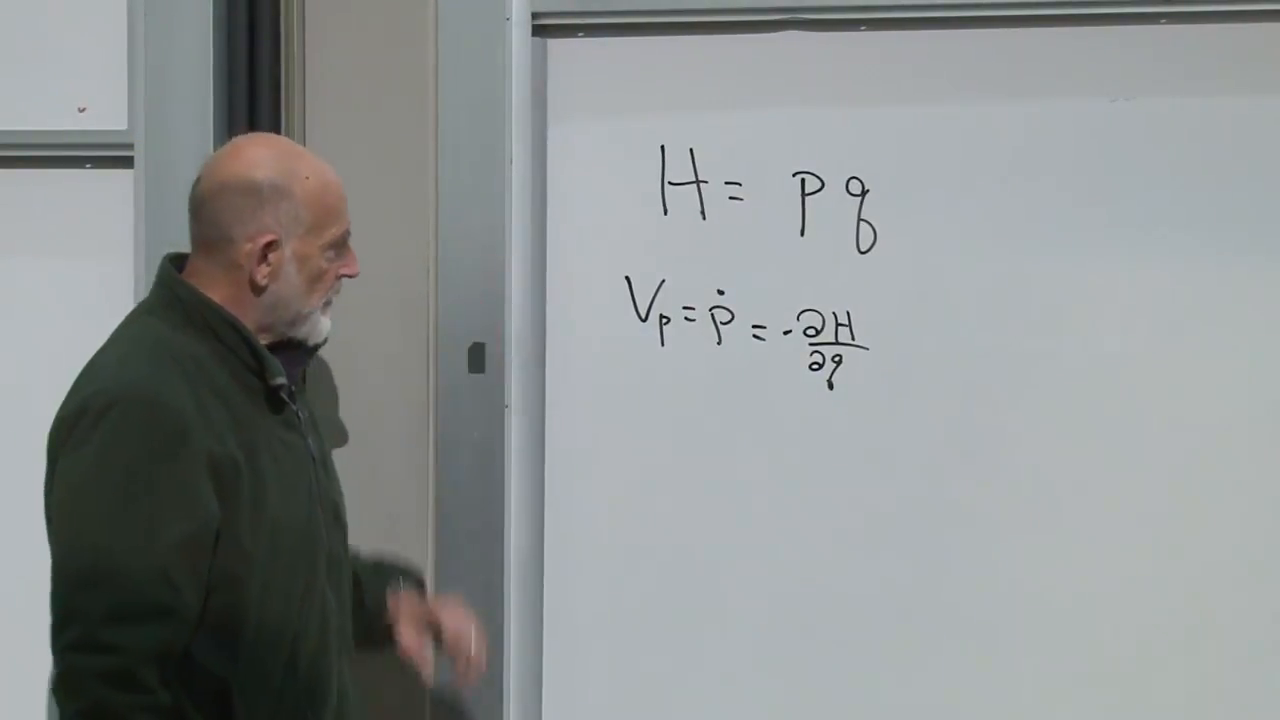
\includegraphics[width=0.82\textwidth]{lecture_07_figure_03.png}
  \caption{Début de l’exemple \(H=pq\) et première composante de la vitesse dans l’espace des phases.}
  \lectureframe{01:00:11}
\end{figure}

Les équations de Hamilton sont
\begin{equation}
  \dot p=-\lambda p,
  \qquad
  \dot q=\lambda q,
  \label{eq:l7-pq-flow}
\end{equation}
et leurs solutions sont
\begin{equation}
  p(t)=p_0e^{-\lambda t},
  \qquad
  q(t)=q_0e^{\lambda t}.
  \label{eq:l7-pq-solutions}
\end{equation}
Un carré est comprimé exponentiellement selon \(p\) et étiré du même facteur selon \(q\) :
\begin{equation}
  \Delta p(t)\Delta q(t)
  =
  \Delta p(0)\Delta q(0).
  \label{eq:l7-pq-area}
\end{equation}
Sa divergence confirme localement le résultat,
\begin{equation}
  \frac{\partial\dot p}{\partial p}
  +\frac{\partial\dot q}{\partial q}
  =-\lambda+\lambda=0.
  \label{eq:l7-pq-divergence}
\end{equation}

\begin{figure}[htbp]
  \centering
  \includegraphics[width=0.86\textwidth]{lecture_07_figure_11.png}
  \caption{Une région compacte étirée en une longue bande mince, tandis que l’aire est préservée par le flot \(H=pq\).}
  \lectureframe{01:02:10}
\end{figure}

\begin{classroomqa}
  \audiencequestion{Puisque \(pq\) a la dimension d’une action, le théorème de Liouville exprime-t-il la conservation de l’action ? \lecturetimestamp{01:03:00--01:04:09}}
  \lecturerresponse{Non. Le théorème exprime la conservation du volume dans l’espace des phases. Pour une paire canonique, \(dq\,dp\) a la dimension d’une action, ce qui annonce la mécanique quantique, où les cellules de l’espace des phases se mesurent en unités déterminées par \(\hbar\). Mais le produit \(pq\) n’est pas en soi la fonctionnelle d’action de Hamilton, et il ne représente pas automatiquement un moment cinétique simplement parce que les dimensions coïncident.}
\end{classroomqa}

Cet exemple montre aussi que les angles ne sont pas nécessairement préservés. Une croix à angle droit, dont les composantes sont inégales, subit un cisaillement dans son aspect métrique lors de la mise à l’échelle décrite par l’équation~\eqref{eq:l7-pq-solutions}, alors que l’aire reste inchangée. Le théorème de Liouville porte sur l’aire ou le volume, et non sur la rigidité au sens de la géométrie euclidienne ordinaire.

\section{L’amortissement crée un puits}

Pour voir ce que le théorème exclut, considérons l’équation réduite d’un oscillateur amorti,
\begin{equation}
  m\ddot x=-kx-c\dot x,
  \qquad c>0.
  \label{eq:l7-damped-newton}
\end{equation}
Posons \(p=m\dot x\). Alors,
\begin{equation}
  \dot x=\frac{p}{m},
  \qquad
  \dot p=-kx-\frac{c}{m}p.
  \label{eq:l7-damped-first-order}
\end{equation}
Sans amortissement, le point représentatif dans l’espace des phases décrit des cercles autour de l’origine. Avec l’amortissement, l’énergie est transférée aux degrés de liberté microscopiques du milieu environnant, et la trajectoire spirale vers l’intérieur.

\begin{figure}[htbp]
  \centering
  \includegraphics[width=0.84\textwidth]{lecture_07_figure_13.png}
  \caption{Équation de l’oscillateur amorti et spirale convergeant vers l’origine dans le plan \(x\)-\(p\).}
  \lectureframe{01:13:30}
\end{figure}

La divergence de ce flot réduit à deux dimensions vaut
\begin{equation}
  \frac{\partial\dot x}{\partial x}
  +\frac{\partial\dot p}{\partial p}
  =
  0-\frac{c}{m}<0.
  \label{eq:l7-damped-divergence}
\end{equation}
Toute région de taille finie se contracte. L’origine est un puits, l’analogue continu de l’application entre états où plusieurs flèches convergent vers un même état.

\begin{figure}[htbp]
  \centering
  \includegraphics[width=0.88\textwidth]{lecture_07_figure_14.png}
  \caption{Composantes de la vitesse dans l’espace des phases de l’oscillateur amorti, utilisées pour obtenir la divergence négative \(-c/m\).}
  \lectureframe{01:16:05}
\end{figure}

Cela ne signifie pas que la mécanique microscopique viole le théorème de Liouville. Les deux variables \(x,p\) laissent de côté l’énorme nombre de degrés de liberté de l’environnement qui reçoivent l’énergie de l’oscillateur. Le système élargi, formé de l’oscillateur et de son environnement, peut être hamiltonien et préserver le volume, même si sa description réduite \(x,p\) implique une contraction.

\begin{classroomqa}
  \audiencequestion{L’oscillateur amorti est-il toujours décrit par l’équation de Newton, même s’il n’est pas hamiltonien dans cet espace des phases réduit ?
  \lecturetimestamp{01:20:09--01:21:12}}
  \lecturerresponse{Oui. La loi \(F=ma\) peut inclure une force de frottement déterminée empiriquement. La description élémentaire fondée sur \(L=T-V\) et la formulation hamiltonienne s’appliquent directement aux forces conservatives ; des lagrangiens plus généraux permettent aussi de traiter certaines forces dépendant de la vitesse. Un terme de frottement markovien pour un système isolé décrit par le couple \(x,p\) relève toutefois d’une dynamique dissipative réduite, et non d’un système hamiltonien canonique fermé.}
\end{classroomqa}

\begin{classroomqa}
  \audiencequestion{Si l’on peut intégrer les équations de l’oscillateur amorti à rebours avec une précision infinie, l’information est-elle vraiment perdue ?
  \lecturetimestamp{01:25:16--01:27:17}}
  \lecturerresponse{Pour tout temps fini, l’équation différentielle idéale admet encore une application inverse : on peut donc remonter le temps à partir de données exactes. L’énoncé précis est que les cellules finies de l’espace des phases se contractent exponentiellement. Pour retrouver leur passé, il faut alors une précision qui augmente exponentiellement ; à temps infini, toutes les trajectoires convergent vers le puits. C’est l’analogue classique continu le plus proche de l’image discrète de la perte de possibilités, et non l’affirmation que deux solutions exactes à temps fini deviennent littéralement une seule.}
\end{classroomqa}

\begin{classroomqa}
  \audiencequestion{Un champ vectoriel peut-il avoir une divergence nulle sans être issu d’un hamiltonien ? \lecturetimestamp{01:18:21--01:22:34}}
  \lecturerresponse{Certainement. La formulation hamiltonienne suffit à assurer une divergence nulle, mais elle n’est pas nécessaire. Un champ de vitesse incompressible quelconque peut avoir une divergence nulle sans être un champ hamiltonien canonique sur ce même espace. Le champ de vitesse d’un fluide incompressible en trois dimensions en est l’exemple classique : trois coordonnées ne peuvent pas, à elles seules, former des paires canoniques. La mécanique complète des fluides peut admettre des formulations hamiltoniennes plus élaborées, en dimension infinie, mais cela ne renverse pas l’implication à sens unique énoncée ici.}
\end{classroomqa}

\section{D’autres distinctions mises en lumière par les questions}

\begin{classroomqa}
  \audiencequestion{Quel est le lien entre le mouvement sur une surface d’énergie constante et la préservation du volume de tout l’espace des phases ?
  \lecturetimestamp{01:28:47--01:30:41}}
  \lecturerresponse{Ce sont des conséquences indépendantes de la structure hamiltonienne. Si \(H\) ne dépend pas explicitement du temps, chaque trajectoire reste sur sa propre surface d’énergie. Une portion finie peut traverser plusieurs de ces surfaces ; le théorème de Liouville affirme que le volume de cette portion entière est préservé. Dans le cas de l’oscillateur harmonique, la portion conserve aussi sa forme, car le flot est une rotation rigide. La portion \(H=pq\) ne conserve que son aire, et non sa forme.}
\end{classroomqa}

\begin{classroomqa}
  \audiencequestion{Quelle place le travail mécanique occupe-t-il dans la formulation hamiltonienne ? \lecturetimestamp{01:30:44--01:32:57}}
  \lecturerresponse{Le travail décrit un transfert d’énergie à travers la frontière choisie d’un système. Un agent extérieur peut soulever un poids ou modifier un paramètre et ainsi changer l’énergie du sous-système ; l’agent perd alors l’énergie qu’il fournit. Si les deux parties sont incluses dans un même modèle fermé, l’accent revient à la conservation de l’énergie totale et aux échanges entre sous-systèmes.}
\end{classroomqa}

\begin{classroomqa}
  \audiencequestion{La préservation du volume implique-t-elle aussi celle de la topologie et des angles ? \lecturetimestamp{01:33:00--01:33:37}}
  \lecturerresponse{Un flot hamiltonien régulier à temps fini préserve la topologie, car il s’agit d’une déformation continue inversible. En général, il ne préserve ni les angles euclidiens ni la forme. La rotation rigide de l’oscillateur les préserve, mais l’étirement dans le cas \(H=pq\) montre pourquoi ce cas est particulier.}
\end{classroomqa}

\begin{classroomqa}
  \audiencequestion{La transformation de Legendre a-t-elle été omise parce qu’elle n’a aucune signification physique ? \lecturetimestamp{01:33:43--01:34:48}}
  \lecturerresponse{Non. C’est la transformation utile qui remplace la description en termes de vitesse par celle en termes de quantité de mouvement et qui produit \(H=\sum_i p_i\dot q_i-L\) lorsque l’application est régulière. Cette construction a déjà été utilisée à plusieurs reprises, même si son nom formel n’a pas été souligné ; la théorie générale détaillée n’est tout simplement pas nécessaire pour le théorème étudié ici.}
\end{classroomqa}

\section{Crochets de Poisson : une nouvelle condensation}

Les dernières minutes reviennent au thème historique. Au XIXe siècle, la mécanique a cherché à plusieurs reprises des structures concises reliant des systèmes apparemment différents --- la mécanique et l’optique géométrique, les particules et les rayons, les trajectoires classiques et les descriptions ondulatoires. Les crochets de Poisson constituent une autre structure de ce type, qui prend une importance particulière en mécanique quantique.

Soit \(F(q,p)\) une fonction quelconque de l’espace des phases. Il peut s’agir d’une coordonnée, d’une quantité de mouvement, du produit \(qp\) ou du moment cinétique. Au cours du mouvement,
\begin{equation}
  \frac{dF}{dt}
  =
  \sum_i\left(
    \frac{\partial F}{\partial q_i}\dot q_i
    +\frac{\partial F}{\partial p_i}\dot p_i
  \right).
  \label{eq:l7-f-time-derivative}
\end{equation}
Substituons les équations de Hamilton :
\begin{equation}
  \frac{dF}{dt}
  =
  \sum_i\left(
    \frac{\partial F}{\partial q_i}
    \frac{\partial H}{\partial p_i}
    -
    \frac{\partial F}{\partial p_i}
    \frac{\partial H}{\partial q_i}
  \right).
  \label{eq:l7-f-hamiltonian-derivative}
\end{equation}

\begin{figure}[htbp]
  \centering
  \includegraphics[width=0.88\textwidth]{lecture_07_figure_15.png}
  \caption{Règle de dérivation en chaîne pour la dérivée temporelle d’une fonction générale de l’espace des phases \(F(q,p)\).}
  \lectureframe{01:42:40}
\end{figure}

La combinaison antisymétrique qui revient ici mérite un nom. Pour deux fonctions quelconques \(F\) et \(G\), définissons leur crochet de Poisson par
\begin{equation}
  \boxed{
  \{F,G\}
  =
  \sum_i\left(
    \frac{\partial F}{\partial q_i}
    \frac{\partial G}{\partial p_i}
    -
    \frac{\partial F}{\partial p_i}
    \frac{\partial G}{\partial q_i}
  \right).}
  \label{eq:l7-poisson-bracket}
\end{equation}

\begin{figure}[htbp]
  \centering
  \includegraphics[width=0.86\textwidth]{lecture_07_figure_16.png}
  \caption{La combinaison de dérivées de deux fonctions, élevée au rang de crochet de Poisson.}
  \lectureframe{01:44:15}
\end{figure}

L’équation~\eqref{eq:l7-f-hamiltonian-derivative} devient
\begin{equation}
  \boxed{\frac{dF}{dt}=\{F,H\}.}
  \label{eq:l7-hamiltonian-poisson-evolution}
\end{equation}
Si \(F\) dépend aussi explicitement du temps, on ajoute \(\partial F/\partial t\). En prenant \(F=q_i\) ou \(F=p_i\), on retrouve les deux équations de Hamilton ; l’équation~\eqref{eq:l7-hamiltonian-poisson-evolution} constitue donc une formulation compacte de la dynamique complète.

On peut toujours condenser artificiellement la notation---on pourrait mettre au carré plusieurs équations, les additionner et appeler le résultat une seule équation. Cela masquerait la structure au lieu de la révéler. Le crochet de Poisson est utile pour la raison inverse : son algèbre organise l’évolution temporelle, les quantités conservées et les symétries. L’étape suivante consiste à développer cette algèbre, puis à l’appliquer au moment cinétique, dont la structure sera centrale en mécanique classique comme en théorie quantique.

\section{Le sens continu de la réversibilité}

Nous pouvons maintenant exposer toute la chaîne d’idées, sans la raccourcir. Les équations de Hamilton conservent \(H\) lorsque l’hamiltonien ne dépend pas explicitement du temps ; les trajectoires individuelles restent donc sur des hypersurfaces d’énergie constante. Ces mêmes équations attribuent une vitesse à chaque point de l’espace des phases. La divergence de ce champ de vitesse est nulle, car les dérivées partielles mixtes s’annulent deux à deux. Par conséquent, une région entière d’états possibles conserve son volume canonique.

C’est la version continue du principe « une flèche entrante, une flèche sortante ». La forme peut changer, les angles peuvent changer et des trajectoires voisines peuvent s’écarter considérablement. Dans une formulation hamiltonienne fermée et régulière, ce qui ne peut pas se produire, c’est la compression d’un ensemble fini de possibilités en un volume plus petit de l’espace des phases. Le flot \(H=pq\) montre qu’il est possible de s’étirer ; l’oscillateur amorti réduit montre le puits qui apparaît dès que les conditions hamiltoniennes ne sont plus satisfaites. Les crochets de Poisson condensent alors la même dynamique en affirmant que l’hamiltonien engendre toute dérivée temporelle.
